\section{Results}
\label{sec:results}

\Cref{tab:main-results} gives the main comparison; the subsections read it experiment by experiment, and \cref{tab:hypotheses} lists the outcome of every prediction.

\subsection{Detection and the limit of the test}
\label{sec:res-detection}

On the six committed tables the twelve identities close with a largest relative residual of \eoneCleanRel{} of the gross total, and none is flagged (\cref{tab:data}).
Planted at \eoneCases{} locations per class, defects of seven classes are flagged in \eoneAboveFullK{} of \eoneAboveFullN{} cases at 1.01 times the limit and in \eoneBelowFullK{} of \eoneBelowFullN{} cases at 0.99 times the limit, over all eight classes: the transition is a step at the limit (\cref{fig:power}a).
The bisected detection limit is the limit itself within \eoneThrDev{} over \eoneBisected{} bisections per class, as Proposition~\ref{prop:limit} states, so on these books a defect is named from \eoneCleanLimitLow{} to \eoneCleanLimitHigh{} USD.
The stage arithmetic and the pooled row detect \eoneAboveStageK{} of the \eoneAboveStageN{} cases, three classes (an allowance movement, an allowance closing and a gross-amount movement), and none of the four classes that live outside the stage tables: an amount reallocated between stages, a waterfall line, the waterfall closing and the stage ECL (\cref{fig:power}b).
The negative control, an amount booked under another line, is flagged in \eoneMisK{} of \eoneMisN{} cases even at one hundred times the limit.

\begin{figure}[htbp]
\centering
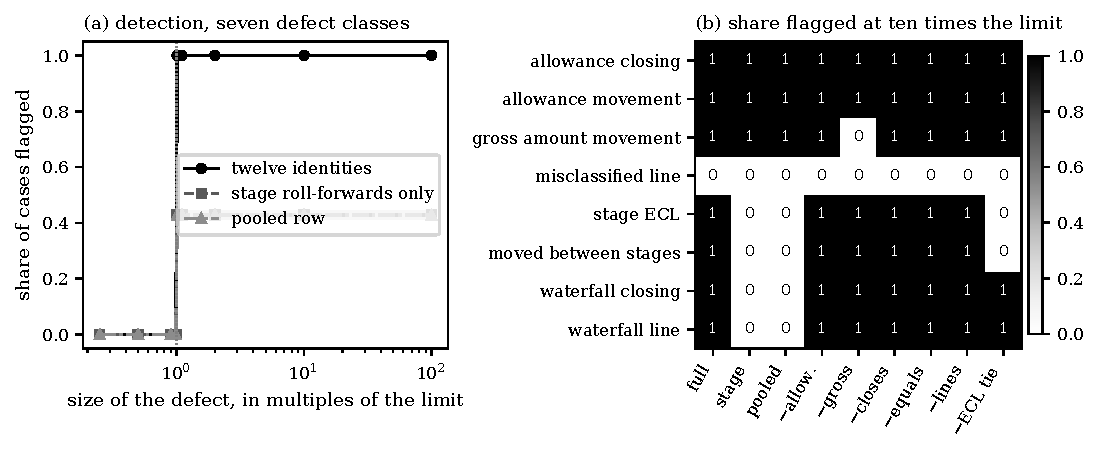
\includegraphics[width=\textwidth]{power}
\caption{Detection of planted defects on the six committed C06 dates. Panel (a) shows the share flagged against the size of the defect in multiples of the limit, pooled over seven defect classes, for the twelve identities, the stage roll-forwards alone and the pooled row, with 95\% Wilson bands. Panel (b) shows the share flagged at ten times the limit, by class and by method, including the full set with one identity family left out.}
\label{fig:power}
\end{figure}

The identities that fail localize the defect to a small group: an allowance movement fails \eoneIdsAllowanceMovement{} identities, an allowance closing \eoneIdsAllowanceClosing{}, a reallocation \eoneIdsStageReallocation{}, a gross-amount movement \eoneIdsGcaMovement{}, a waterfall line \eoneIdsWaterfallLine{}, the waterfall closing \eoneIdsWaterfallClosing{} and a stage ECL \eoneIdsStageEcl{}.
\Cref{fig:incidence} shows the matrix behind this: every entry is seen by at least one equation, the \esixEntries{} entries fall in \esixPatterns{} patterns, and the rank is \esixRank{}.

\begin{figure}[htbp]
\centering
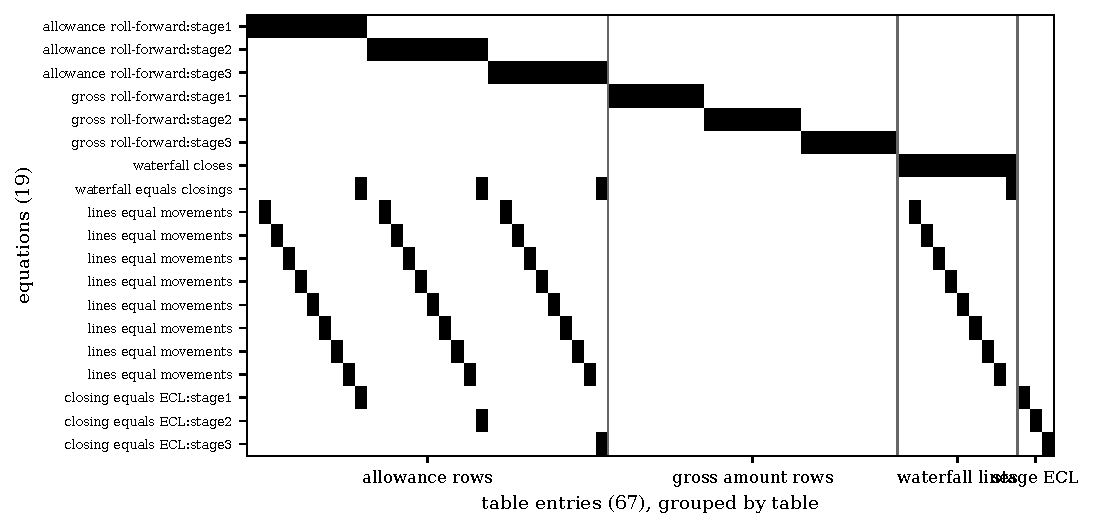
\includegraphics[width=\textwidth]{incidence}
\caption{Absolute value of the signed matrix of the identities for the 2008-12 book: 19 equations in rows and 67 table entries in columns, grouped by table. A dark cell means the entry appears in the equation. Entries with identical columns cannot be told apart by the failing identities.}
\label{fig:incidence}
\end{figure}

\subsection{Tolerance basis and rounding}
\label{sec:res-rounding}

An absolute tolerance of $10^{-6}$ units flags \etwoAbsCommittedK{} of the six clean committed tables and \etwoAbsResK{} of \etwoResN{} resampled books (\etwoAbsResPct{}, Wilson 95\% interval \etwoAbsResLo{} to \etwoAbsResHi{}); absolute tolerances of 0.01 and 1 units, and every relative tolerance from $10^{-12}$ to $10^{-4}$, flag none.
The largest relative residual of a resampled book is \etwoRelMaxResid{}, so the choice of $10^{-6}$ is nine orders above the noise and the tolerance is a policy value, not a numerical necessity.
After rounding every stored number (\cref{tab:rounding}, \cref{fig:rounding}), no book is flagged at units of 1, 10 and 1,000, and \etwoRoundTenThousandK{} of \etwoResN{} at 10,000, as Proposition~\ref{prop:rounding} requires.
At 100,000 units \etwoRoundHundredThousandPct{} are flagged (interval \etwoRoundHundredThousandLo{} to \etwoRoundHundredThousandHi{}), from \etwoHundredLow{} to \etwoHundredHigh{} by date, lower on the larger books whose limit is larger.
At one million units \etwoRoundMillionK{} are flagged (\etwoRoundMillionPct{}, \etwoRoundMillionLo{} to \etwoRoundMillionHi{}); the prediction of more than 99\% was refuted.
The \etwoMillionUnflagged{} books not flagged are spread over the six dates (\etwoMillionUnflaggedDates{}), and the cause is not established.

\begin{figure}[htbp]
\centering
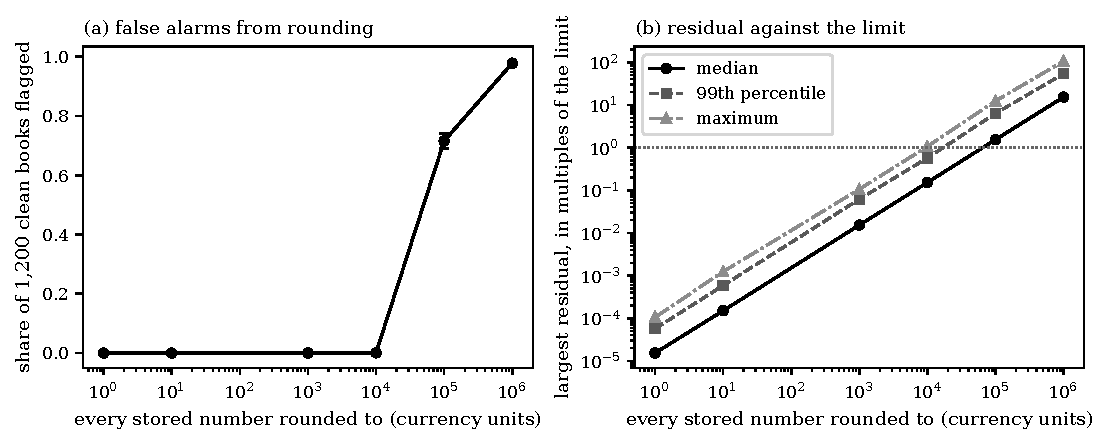
\includegraphics[width=\textwidth]{rounding}
\caption{Rounding of clean resampled books. Panel (a) shows the share of the 1,200 books flagged against the unit to which every stored number is rounded, with Wilson intervals. Panel (b) shows the median, 99th percentile and maximum over books of the largest residual in multiples of the limit; the dotted line at one is the flagging threshold.}
\label{fig:rounding}
\end{figure}

\begin{table}[htbp]
\centering
\small
\caption{False alarms of the test on 1,200 clean resampled books after every stored number is rounded independently to the stated unit: books flagged, and the largest residual of a book as a multiple of the limit (median, 99th percentile and maximum over the books; a value above 1 is a flag).}
\label{tab:rounding}
\begin{adjustbox}{max width=\textwidth}
\begin{tabular}{lrrrrr}
\toprule
Rounded to (units) & Flagged & Percent [Wilson 95\%] & Median & 99th percentile & Maximum \\
\midrule
1 & 0/1,200 & 0.0 [0.0, 0.3] & 0.000 & 0.000 & 0.00 \\
10 & 0/1,200 & 0.0 [0.0, 0.3] & 0.000 & 0.001 & 0.00 \\
1,000 & 0/1,200 & 0.0 [0.0, 0.3] & 0.015 & 0.062 & 0.11 \\
10,000 & 1/1,200 & 0.1 [0.0, 0.5] & 0.152 & 0.572 & 1.06 \\
100,000 & 859/1,200 & 71.6 [69.0, 74.1] & 1.539 & 6.321 & 12.35 \\
1,000,000 & 1,174/1,200 & 97.8 [96.8, 98.5] & 15.255 & 53.850 & 105.91 \\
\bottomrule
\end{tabular}
\end{adjustbox}
\end{table}


\subsection{Overlays}
\label{sec:res-overlays}

In \ethreeSets{} overlay sets drawn at random the model ECL and the ECL by stage never changed and the total was always the model ECL plus the overlays: \ethreeViolations{} violations.
\Cref{tab:placement} gives the placement: the correct booking closes every identity in all \ethreeCases{} cases; the four wrong bookings that put the overlay in some tables and not in others are flagged by the twelve identities in all \ethreeCases{} cases each, by \ethreeIdsNotCarried{}, \ethreeIdsWrongStage{}, \ethreeIdsDoubleCarried{} and \ethreeIdsCarriedNotInWaterfall{} identities, and by neither the stage arithmetic nor the pooled row.
The overlay merged into the model ECL under the remeasurement line closes every identity and is flagged by nothing.
On the synthetic bank the two committed overlays are \ethreeSevenOverlay{} million CLP of an allowance of \ethreeSevenAllowance{} million, \ethreeSevenShare{}, and a merge would overstate the model ECL by \ethreeSevenMerge{}.

\begin{table}[htbp]
\centering
\small
\caption{Six ways to book an overlay of 2\%, 10\% and 25\% of the allowance on each of the six committed dates (18 cases per row): cases flagged by the twelve identities, by the two roll-forwards of each stage alone and by one pooled row, and the number of identities that fail when the booking is flagged.}
\label{tab:placement}
\begin{adjustbox}{max width=\textwidth}
\begin{tabular}{p{6.6cm}rrrr}
\toprule
Booking of an overlay & Twelve identities & Stage arithmetic & Pooled row & Identities failing \\
\midrule
Carried in the stage 1 row, no waterfall line & 18/18 & 0/18 & 0/18 & 3 \\
Correct booking (stage 1 row, waterfall line, both closings) & 0/18 & 0/18 & 0/18 & 0 \\
Carried in stage 1 and stage 2 rows, one waterfall line & 18/18 & 0/18 & 0/18 & 3 \\
Added to the model ECL under the remeasurement line & 0/18 & 0/18 & 0/18 & 0 \\
Waterfall only, stage rows untouched & 18/18 & 0/18 & 0/18 & 3 \\
Carried in the stage 2 row, waterfall line at portfolio level & 18/18 & 0/18 & 0/18 & 2 \\
\bottomrule
\end{tabular}
\end{adjustbox}
\end{table}


\subsection{Non-linearity of the weighted PD}
\label{sec:res-nonlinearity}

Of \efourDraws{} draws, \efourConvexN{} have every factor in the convex region and none has a negative index (smallest \efourConvexMin{}); \efourConcaveN{} have every factor in the concave region and none has a positive index (largest \efourConcaveMax{}); \efourMixedN{} are mixed, with \efourMixedPos{} positive and \efourMixedNeg{} negative indexes, down to \efourMixedMin{} (\cref{fig:sweep}).
The Gauss--Hermite check of the engine is within \efourGhErr{} in every draw.
The second-order formula is within 25\% of the index in \efourSecondWithin{} of \efourSecondN{} convex draws, with a median ratio of \efourSecondQFifty{} and 5th to 95th percentiles of \efourSecondQFive{} to \efourSecondQNinetyFive{}.

\begin{figure}[htbp]
\centering
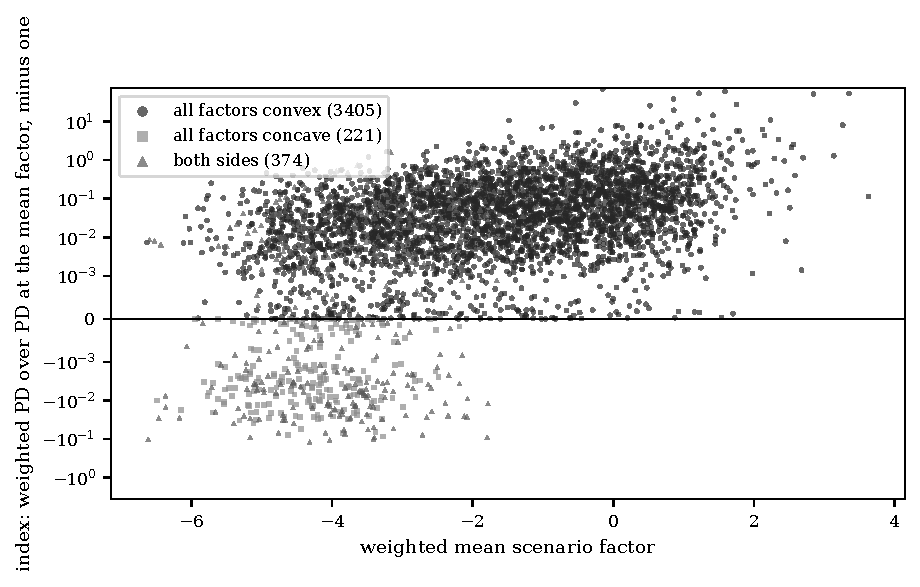
\includegraphics[width=0.85\textwidth]{sweep}
\caption{Index of the weighted PD against the weighted mean scenario factor for the first 4,000 draws of the sweep, by position of the scenario factors relative to the inflection of the conditional PD; the vertical axis is symmetric logarithmic and the horizontal line marks zero.}
\label{fig:sweep}
\end{figure}

On the six committed dates (\cref{tab:committed-nonlinearity}) every scenario lies in the convex region, the inflection is between \efourZstarLow{} and \efourZstarHigh{} and the lowest factor is \efourZminLow{} or higher, the PD-level index runs from \efourPdLow{} to \efourPdHigh{}, and the engine reproduces it to \efourPdAgree{}.
The ECL-level index is positive on \efourEclPositive{} of six dates and \efourEclTen{} on 2010-12, where the Stage 2 share is \efourTenShare{} and the Stage 2 ratio differs by \efourGapTen{} between recomputed and frozen staging, against at most \efourGapOther{} on the other dates.
Staging that responds to the weights is the one feature that distinguishes that date; we did not isolate it as the cause.

\begin{table}[htbp]
\centering
\small
\caption{The six committed C06 dates: the inflection of the conditional PD, the lowest and highest scenario factor, the PD-level index recomputed by the engine from the committed scenario factors (equal to the committed value), the committed ECL-level index, the Stage 2 share of the gross amount and the gap between the Stage 2 ratio under recomputed and frozen staging at the grid weights nearest to the committed ones.}
\label{tab:committed-nonlinearity}
\begin{adjustbox}{max width=\textwidth}
\begin{tabular}{lrrrrrrr}
\toprule
Date & Inflection $z^*$ & Lowest $z$ & Highest $z$ & PD-level index & ECL-level index & Stage 2 share & Stage 2 gap \\
\midrule
2006-12 & -6.41 & -0.99 & -0.81 & 0.00113 & +0.00211 & 0.1\% & 0.00005 \\
2008-12 & -6.16 & -1.48 & -1.35 & 0.00079 & +0.02121 & 1.1\% & 0.00009 \\
2010-12 & -5.73 & -2.46 & -1.61 & 0.01882 & -0.00071 & 56.5\% & 0.01510 \\
2019-12 & -5.74 & -0.01 & 0.50 & 0.01164 & +0.02320 & 0.0\% & 0.00000 \\
2020-06 & -5.75 & -2.15 & -2.07 & 0.00017 & +0.01279 & 96.7\% & 0.00007 \\
2023-06 & -5.82 & 0.03 & 0.30 & 0.00323 & +0.00622 & 0.0\% & 0.00002 \\
\bottomrule
\end{tabular}
\end{adjustbox}
\end{table}


Against the full distribution of the factor (\cref{tab:designs}, \cref{fig:designs}) the base scenario alone has a median absolute error of \efourSingleMed{} (\efourSingleMedLo{} to \efourSingleMedHi{}), three scenarios at one standard deviation \efourAdhocMed{}, tertile means \efourTertileMed{}, the three-point rule \efourGhThreeMed{} and the five-point rule \efourGhFiveMed{}.
Among the \efourStrong{} draws with a margin of two standard deviations inside the convex region, the base scenario and the 25/50/25 set understate the expected PD in \efourSingleUnder{} and \efourAdhocUnder{}; the median ratio of the predicted to the measured bias of the 25/50/25 set is \efourBiasMedian{}.

\begin{figure}[htbp]
\centering
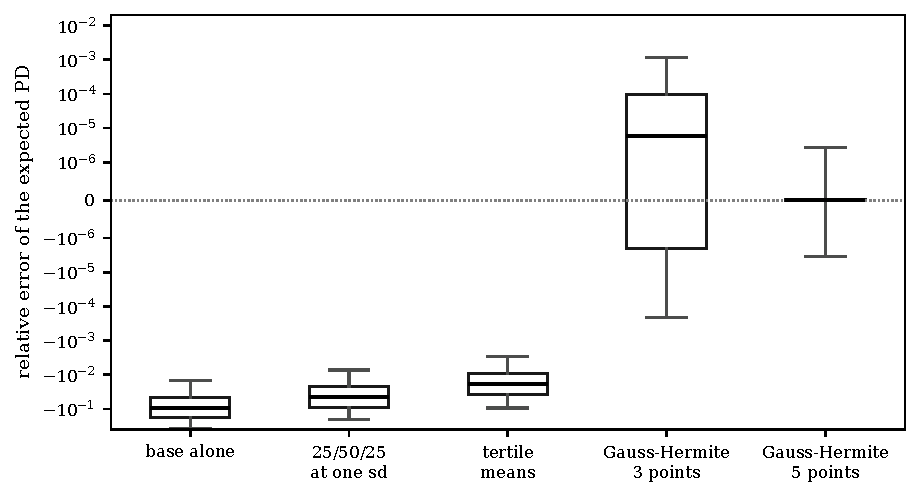
\includegraphics[width=0.85\textwidth]{designs}
\caption{Relative error of the expected PD for five scenario sets against the 64-node Gauss--Hermite expectation, over 5,000 draws: boxes span the quartiles, whiskers the 5th and 95th percentiles, the thick line is the median; the axis is symmetric logarithmic.}
\label{fig:designs}
\end{figure}

\begin{table}[htbp]
\centering
\small
\caption{Relative error of the expected PD of five scenario sets against the 64-node Gauss--Hermite expectation under a normal factor, over 5,000 draws of the PD, the correlation and the forecast mean and spread: quantiles of the signed error in percent, the share of draws with absolute error above 5\%, and the share understated among the draws whose forecast lies two standard deviations inside the convex region.}
\label{tab:designs}
\begin{adjustbox}{max width=\textwidth}
\begin{tabular}{p{5.2cm}rrrrr}
\toprule
Scenario set & 5th pct (\%) & Median (\%) & 95th pct (\%) & $|$error$|>5\%$ & Understated (convex margin) \\
\midrule
Base scenario alone & -38 & -9.2 & -1.47 & 72.4\% & 100.0\% \\
Three scenarios at one standard deviation, 25/50/25 & -19.9 & -4.56 & -0.727 & 46.4\% & 100.0\% \\
Three equal-probability tertile means & -9.4 & -1.84 & -0.293 & 16.7\% & 100.0\% \\
Three-point Gauss--Hermite & -0.0211 & +0.0006 & +0.119 & 0.0\% & 29.2\% \\
Five-point Gauss--Hermite & -0.000336 & +4.27e-09 & +0.000267 & 0.0\% & 41.1\% \\
\bottomrule
\end{tabular}
\end{adjustbox}
\end{table}


\subsection{Three regimes on one synthetic bank}
\label{sec:res-regimes}

\Cref{tab:regimes} and \cref{fig:regimes} give the committed totals and the ten-seed ratios.
The committed base scenario has B-1 \efiveCommittedBaseB{}, IFRS 9 \efiveCommittedBaseI{} and Annex 9 \efiveCommittedBaseA{} billion CLP; the combined severe scenario \efiveCommittedCombinedB{}, \efiveCommittedCombinedI{} and \efiveCommittedCombinedA{}.
The committed seed is reproduced to \efiveCommittedDiff{} currency units.
Over \efiveSeeds{} seeds the IFRS 9 over B-1 ratio is \efiveBaseMean{} in the base (95\% interval \efiveBaseLo{} to \efiveBaseHi{}, standard deviation \efiveBaseSd{}) and \efiveCombinedMean{} in the combined severe scenario (\efiveCombinedLo{} to \efiveCombinedHi{}); it is below one in the other five scenarios and above one in the severe one \efiveOrder{}.
IFRS 9 exceeds Annex 9 in the base in \efiveIfrsAboveBde{} seeds of \efiveSeeds{}.
The bridge closes within \efiveBridgeMax{} units in all \efiveCells{} runs and the engine's reconciliation test is green in \efiveGreen{} of them.
In the base the mean steps are $\efiveStepBaseMeasurementBasis$ billion for the measurement basis, $+\efiveStepBaseLifetimeHorizon$ for the lifetime horizon, $+\efiveStepBaseForwardLooking$ for probability weighting, $+\efiveStepBaseDiscounting$ for discounting and $+\efiveStepBaseIfrsNineOverlays$ for overlays; the B-1 minimum is not binding.
The non-linearity index of the IFRS 9 allowance averages \efiveNlBase{} (\efiveNlBaseLow{} to \efiveNlBaseHigh{}) in the base.

\begin{figure}[htbp]
\centering
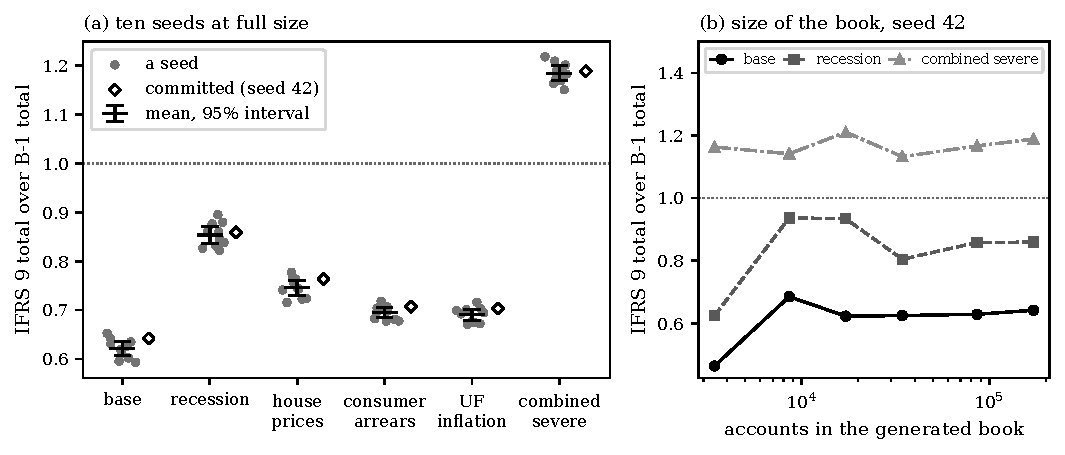
\includegraphics[width=\textwidth]{regimes}
\caption{IFRS 9 total over B-1 total of the synthetic bank. Panel (a) shows, for each scenario, the ten seeds at full size (grey dots), their mean with a 95\% interval and the committed seed 42 (diamond). Panel (b) shows seed 42 at six sizes of the generated book; the dotted line at one marks equal totals.}
\label{fig:regimes}
\end{figure}

\begin{table}[htbp]
\centering
\small
\caption{The three provisioning regimes on the synthetic Banco Andino in six scenarios: the committed totals (seed 42, full size), their ratio, and the mean over ten seeds at full size of the IFRS 9 and Annex 9 totals over the B-1 total with the 95\% $t$ interval of the mean in brackets.}
\label{tab:regimes}
\begin{adjustbox}{max width=\textwidth}
\begin{tabular}{lrrrrrr}
\toprule
Scenario & B-1 (CLP bn) & IFRS 9 (CLP bn) & Annex 9 (CLP bn) & IFRS 9/B-1 & IFRS 9/B-1, ten seeds & Annex 9/B-1, ten seeds \\
\midrule
Base & 152.0 & 97.6 & 79.6 & 0.642 & 0.621 [0.606, 0.635] & 0.549 [0.532, 0.566] \\
Recession & 197.5 & 169.8 & 116.3 & 0.860 & 0.854 [0.836, 0.871] & 0.601 [0.584, 0.618] \\
House price fall & 168.9 & 128.8 & 94.6 & 0.763 & 0.746 [0.731, 0.760] & 0.599 [0.581, 0.617] \\
Consumer arrears shock & 178.6 & 126.3 & 97.3 & 0.707 & 0.694 [0.684, 0.705] & 0.581 [0.566, 0.596] \\
UF inflation spike & 166.9 & 117.4 & 85.6 & 0.703 & 0.690 [0.679, 0.701] & 0.552 [0.536, 0.568] \\
Combined severe & 275.8 & 327.8 & 191.6 & 1.189 & 1.185 [1.170, 1.200] & 0.699 [0.679, 0.719] \\
\bottomrule
\end{tabular}
\end{adjustbox}
\end{table}


The ratios depend on the size of the book (\cref{tab:ladder}): at \efiveLadderLowAccounts{} accounts the base ratio is \efiveLadderLowBase{} against \efiveLadderHighBase{} at full size, while the combined severe ratio is above one at \efiveLadderSevereAbove{} of \efiveLadderCount{} sizes.

\begin{table}[htbp]
\centering
\small
\caption{The IFRS 9 total over the B-1 total of the synthetic bank at seed 42 for six sizes of the generated book (the size factor scales every portfolio's account count), with the largest bridge residual over the six scenarios in currency units and the measured time of one build of the six scenarios.}
\label{tab:ladder}
\begin{adjustbox}{max width=\textwidth}
\begin{tabular}{rrrrrrr}
\toprule
Size factor & Accounts & Base & Recession & Combined severe & Bridge residual & Seconds \\
\midrule
0.02 & 3,430 & 0.464 & 0.625 & 1.163 & 2.4e-07 & 4 \\
0.05 & 8,575 & 0.685 & 0.937 & 1.142 & 7.2e-07 & 5 \\
0.1 & 17,150 & 0.623 & 0.934 & 1.211 & 3.8e-06 & 16 \\
0.2 & 34,300 & 0.625 & 0.805 & 1.133 & 3.8e-06 & 37 \\
0.5 & 85,750 & 0.629 & 0.858 & 1.167 & 2.3e-05 & 86 \\
1 & 171,500 & 0.642 & 0.860 & 1.189 & 3.1e-05 & 56 \\
\bottomrule
\end{tabular}
\end{adjustbox}
\end{table}


\subsection{Outcome of the predictions}
\label{sec:res-hypotheses}

\hypHeld{} of \hypTotal{} predictions held and \hypRefuted{} were refuted: \hypRefutedList{}.
The rounding to millions (Q3b), the one blind entry (A2) and the group of eleven entries (A4) were wrong in their numbers; the weighted ECL above the mean path on every committed date (S3) is contradicted by 2010-12.

\begin{table}[htbp]
\centering
\small
\caption{Main comparison of the proposed protocol with the comparators run on the same data: detection of planted defects by the twelve identities, the stage arithmetic and the pooled row; false alarms on clean tables by tolerance basis; overlay bookings; the non-linearity of the weighted PD; the error of short scenario sets against the full distribution of the factor; and the three regimes of the synthetic bank over ten seeds. Intervals as stated in the last column.}
\label{tab:main-results}
\begin{adjustbox}{max width=\textwidth}
\begin{tabular}{p{5.4cm}p{3.3cm}p{4.0cm}p{3.0cm}}
\toprule
Measurement & Proposed protocol & Comparator & Uncertainty \\
\midrule
Detection above the limit (1.01 times), seven defect classes, 600 cases each & 4,200/4,200 [99.9, 100.0] & stage 1,800/4,200 [41.4, 44.4]; pooled 1,800/4,200 [41.4, 44.4] & Wilson 95\% interval, percent \\
Detection below the limit (0.99 times), eight classes & 0/4,800 [0.0, 0.1] & stage 0/4,800; pooled 0/4,800 & Wilson 95\% interval, percent \\
Smallest defect named, as a multiple of the limit, 120 bisections per class & 1 within $2.4\times10^{-10}$ & not applicable (no comparator names a size) & largest deviation over 840 bisections \\
Clean committed tables flagged (six dates) & 0/6 (relative 1e-6) & 4/6 (absolute 1e-6) & count, no sampling \\
Clean resampled books flagged (1,200) & 0/1,200 [0.0, 0.3] & absolute 1e-6: 68/1,200 [4.5, 7.1] & Wilson 95\% interval, percent \\
Wrong overlay bookings detected (four kinds, 18 cases each) & 72/72 & stage 0/72; pooled 0/72 & count over the full enumeration \\
Negative index among draws in the convex region & 0/16,906 & unqualified statement fails in 1,844/20,000 draws & count over the sweep \\
Median absolute error of the expected PD, base scenario alone & not applicable & 9.20\% [8.94, 9.54] & bootstrap 95\% interval \\
Median absolute error, three scenarios at one standard deviation, 25/50/25 & not applicable & 4.56\% [4.41, 4.75] & bootstrap 95\% interval \\
Median absolute error, three equal-probability tertile scenarios & not applicable & 1.84\% [1.77, 1.92] & bootstrap 95\% interval \\
Median absolute error, three-point Gauss--Hermite scenarios & not applicable & $3.0\times10^{-3}$\% [$2.7\times10^{-3}$, $3.4\times10^{-3}$] & bootstrap 95\% interval \\
IFRS 9 over B-1, base scenario, ten seeds & 0.621 [0.606, 0.635] & B-1 is the reference (1) & mean and 95\% $t$ interval \\
IFRS 9 over B-1, combined severe scenario, ten seeds & 1.185 [1.170, 1.200] & B-1 is the reference (1) & mean and 95\% $t$ interval \\
Largest bridge residual, 60 runs (currency units) & $3.8\times10^{-5}$ & not applicable & maximum, no sampling \\
\bottomrule
\end{tabular}
\end{adjustbox}
\end{table}

\begin{longtable}{lp{7.6cm}p{4.4cm}}
\caption{The 31 statements tested by the experiments, each stated in the header of its script, with what the header and the history of the design document say about when it was set; the repository does not record whether a prediction preceded the first run of its script. The 27 statements whose result no committed document held are predictions; the 4 others (B6, C1, C2, C3) are reproductions and are not counted as predictions.}\label{tab:hypotheses}\\
\toprule
ID & Statement & Set \\
\midrule
\endfirsthead
\toprule
ID & Statement & Set \\
\midrule
\endhead
\bottomrule
\endfoot
P1 & The smallest defect the test names equals the limit for every class but the misclassification. & stated in the script header; the notebook had measured it on one defect class \\
P2 & The pooled row and the stage arithmetic detect three classes above the limit and none of the other four; the twelve identities detect all seven. & stated in the script header \\
P3 & Leaving out one identity family loses a class entirely for exactly two families: the gross amount roll-forward and the tie to the ECL. & stated in the script header \\
Q1 & An absolute tolerance of 1e-6 units flags a clean committed table; the relative basis flags none of the six or of the 1,200 resampled books. & stated in the script header; the notebook had measured the flag on a committed table \\
Q2 & After rounding to 1, 10 and 1,000 units no book is flagged; at 10,000 fewer than 1\% are. & stated in the script header \\
Q3a & After rounding to 100,000 units between 30\% and 95\% of the books are flagged. & stated in the script header \\
Q3b & After rounding to 1,000,000 units more than 99\% of the books are flagged. & stated in the script header \\
O1 & The model ECL does not depend on the overlays and the total is the model ECL plus the overlays, in 3,000 draws. & stated in the script header \\
O2 & The correct overlay booking closes every identity in 18 of 18 cases. & stated in the script header \\
O3 & The twelve identities flag four wrong overlay bookings in 18 of 18 cases each; the stage arithmetic and the pooled row flag none. & stated in the script header \\
O4 & No method flags an overlay merged into the model ECL. & stated in the script header \\
N1 & No negative index among the draws whose factors all lie in the convex region. & stated in the script header; the notebook had swept another seed \\
N2 & No positive index among the draws whose factors all lie in the concave region, with at least 100 such draws. & stated in the script header \\
N3 & Both signs occur among the draws with factors on both sides of the inflection. & stated in the script header \\
N4 & The second-order formula is within 25\% of the index in at least 75\% of the convex draws. & stated in the script header \\
R1 & Where the forecast lies two standard deviations inside the convex region the base scenario alone understates the expected PD in at least 99\% of the draws. & stated in the script header \\
R2 & The median absolute error is ordered gh5 < gh3 < tertile3 < adhoc3 < single. & stated in the script header \\
R3 & The second-order bias of the three-scenario set is within 20\% of the measured bias at the median. & stated in the script header \\
B1 & The bridge closes to within one currency unit in every seed and scenario. & stated in the script header \\
B2 & The engine's reconciliation test is green in every seed and scenario. & stated in the script header \\
B3 & IFRS 9 is below B-1 in five scenarios and above it in the combined severe scenario, in every seed. & stated in the script header \\
B4 & IFRS 9 is above Annex 9 in the base scenario in at least 8 of 10 seeds. & stated in the script header \\
B5 & The standard deviation over seeds of the base IFRS 9 over B-1 ratio is below 0.05. & stated in the script header \\
B6 & The committed seed at the committed size reproduces every committed regime total to within one currency unit (reproduction of the committed totals). & after the bake; the committed totals had been read \\
A1 & The engine's residuals equal the signed map times the perturbation for every entry of the six dates. & stated in the script header \\
A2 & Exactly one entry is seen by no identity: the model ECL of the POCI stage. & stated in the script header \\
A3 & The signed map has full row rank. & stated in the script header \\
A4 & The largest group of entries no failing pattern distinguishes has at least 11 entries. & stated in the script header \\
C1 & The reference example gives a weighted PD of 2.68\% against 1.80\% at the mean factor (reproduction of the acceptance criterion). & before the bake (design document, 5 October 2026); the bake was built to meet it \\
C2 & The identities close on the tolerance basis on the six committed dates (reproduction of the acceptance criterion). & before the bake (design document, 5 October 2026); the bake was built to meet it \\
C3 & The weighted ECL exceeds the ECL at the mean path on every committed date (stated in the product as not claimed). & after the bake; stated in the product as not claimed \\
\end{longtable}

\begin{table}[htbp]
\centering
\small
\caption{The six committed reporting dates of the SBA 7(a) loan book: the gross carrying amount G, the limit of the test on the engine's tolerance basis, the share of the gross amount in Stage 2, the number of loans in the staged book and the largest residual of the twelve identities on the committed tables.}
\label{tab:data}
\begin{adjustbox}{max width=\textwidth}
\begin{tabular}{lrrrrr}
\toprule
Date & Gross amount G (USD bn) & Limit $10^{-6}G$ (USD) & Stage 2 share & Loans & Largest residual (USD) \\
\midrule
2006-12 & 47.1 & 47,124 & 0.1\% & 305,319 & $1.5\times10^{-5}$ \\
2008-12 & 47.2 & 47,248 & 1.1\% & 311,503 & $1.2\times10^{-7}$ \\
2010-12 & 55.5 & 55,460 & 56.5\% & 280,265 & $3.8\times10^{-6}$ \\
2019-12 & 99.6 & 99,603 & 0.0\% & 271,801 & $1.5\times10^{-5}$ \\
2020-06 & 99.7 & 99,711 & 96.7\% & 268,493 & $1.3\times10^{-5}$ \\
2023-06 & 116.8 & 116,761 & 0.0\% & 251,636 & $1.2\times10^{-7}$ \\
\bottomrule
\end{tabular}
\end{adjustbox}
\end{table}

